For this lab we want you to create a wave effect across the 16 LEDs on the Basys 3 board. The idea is to make the LEDs increase and decrease in brightness with some form of pattern. This will require modifying the top level to instantiate additional copies of the PWM module to drive the other LEDs and the creation of a slow clock to cycle the duty values for creating the effect. 

\raggedright

\subsection{Python Test bench Tool}
To make life easier when testing your design we have put together a testing tool to visualize the light levels of the LEDs based on the simulation outputs. An example text file has been produced by running the provided top-level test bench. The code for the python script has been provided, and anyone wanting to run it can. Ensure the file is in the same directory as the \textit{leds.txt} and ensure that you have the opencv libraries installed. You can also go to \url{\ledvisualzationurl}. This server should be available to anyone connected to the U of C network, either directly or through the U of C VPN. If the server goes down, send an email to \labInstructorEmail and I will bring it back up as soon as possible. 
\begin{verbatim}
function void print_leds_to_file(input bit [15:0] LEDS, input integer file_descriptor);
    integer i;
    string led_values;

    // Check if the file is open
    if (file_descriptor == 0) begin
        $display("Error: File is not open!");
        return;
    end

    // Initialize the led_values string
    led_values = "";
    // Iterate through the LEDS array and append the binary values to the led_values string
    for (i = 0; i < 16; i++) begin
        led_values = {led_values, $sformatf("%b", LEDS[i])};
    end
    $timeformat(-3,10,"");
    $fwrite(file_descriptor, "%0t %s\n", $realtime, led_values);
    
endfunction

always@(led) begin
    $display("led = %b", led);
    print_leds_to_file({led,15'b000000000000000}, file_descriptor);
end

  initial begin   
    file_descriptor = $fopen("leds.txt", "w");
    // ... The rest of your testbench
    // Close the output file
     $fclose(file_descriptor);
    // Finish the simulation
    $finish;
  end
\end{verbatim}

\normalsize
The above code is present in the top level test bench file and is responsible for producing the \textit{leds.txt} which contains the printed LED values alongside the time of that value. Proceed to the led visualization url and use the file to see an approximation of how the leds will appear. 

\begin{figure}[H]
    \centering
    
\includegraphics[width=9cm]{Images/ProvidedPWM/LED_VisualizationTool.jpg}
    \caption{LED Visualization Tool}
    \label{fig:enter-label}
\end{figure}
The visualization tool is fairly simple. Click upload file and select the leds.txt file which was created when you ran the simulation. Then press the upload button. The upload will run, and a short video file will be returned.\textit{Generating the video file can take up to 5 minutes for periods of roughly 1 second!} The video will look somewhat like the following.
\begin{figure}[H]
    \centering
    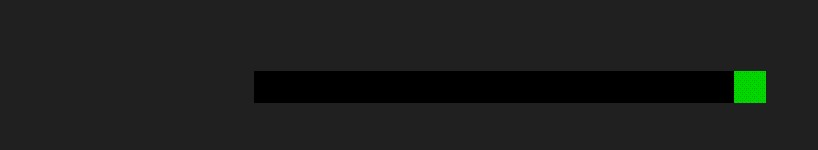
\includegraphics[height=1cm]{Images/ProvidedPWM/SingleLEDFlashing.jpg}
    \caption{Single LED Output}
    \label{fig:enter-label}
\end{figure}
There will be a single blinking square on the right hand side of the image. This is because only 1 led is changing values in the current setup.
